\vspace{-0.1in}
\section{\env}
\label{sec:generation}
\vspace{-0.1in}

\env is a framework to procedurally generate \eai environments. It extends \thor and, thereby, inherits \thor's large asset library, robotic agents, and accurate physics simulation. Just as in scenes painstakingly created by designers in \thor, environments in \env are fully interactive and support navigation, object manipulation, and multi-agent interaction.

\begin{minipage}{\linewidth}
    \centering
    \vspace{0.05in}
    \begin{overpic}[width=\textwidth]{figures/compressions/generation-3-raster.jpg}
        \put(0,0){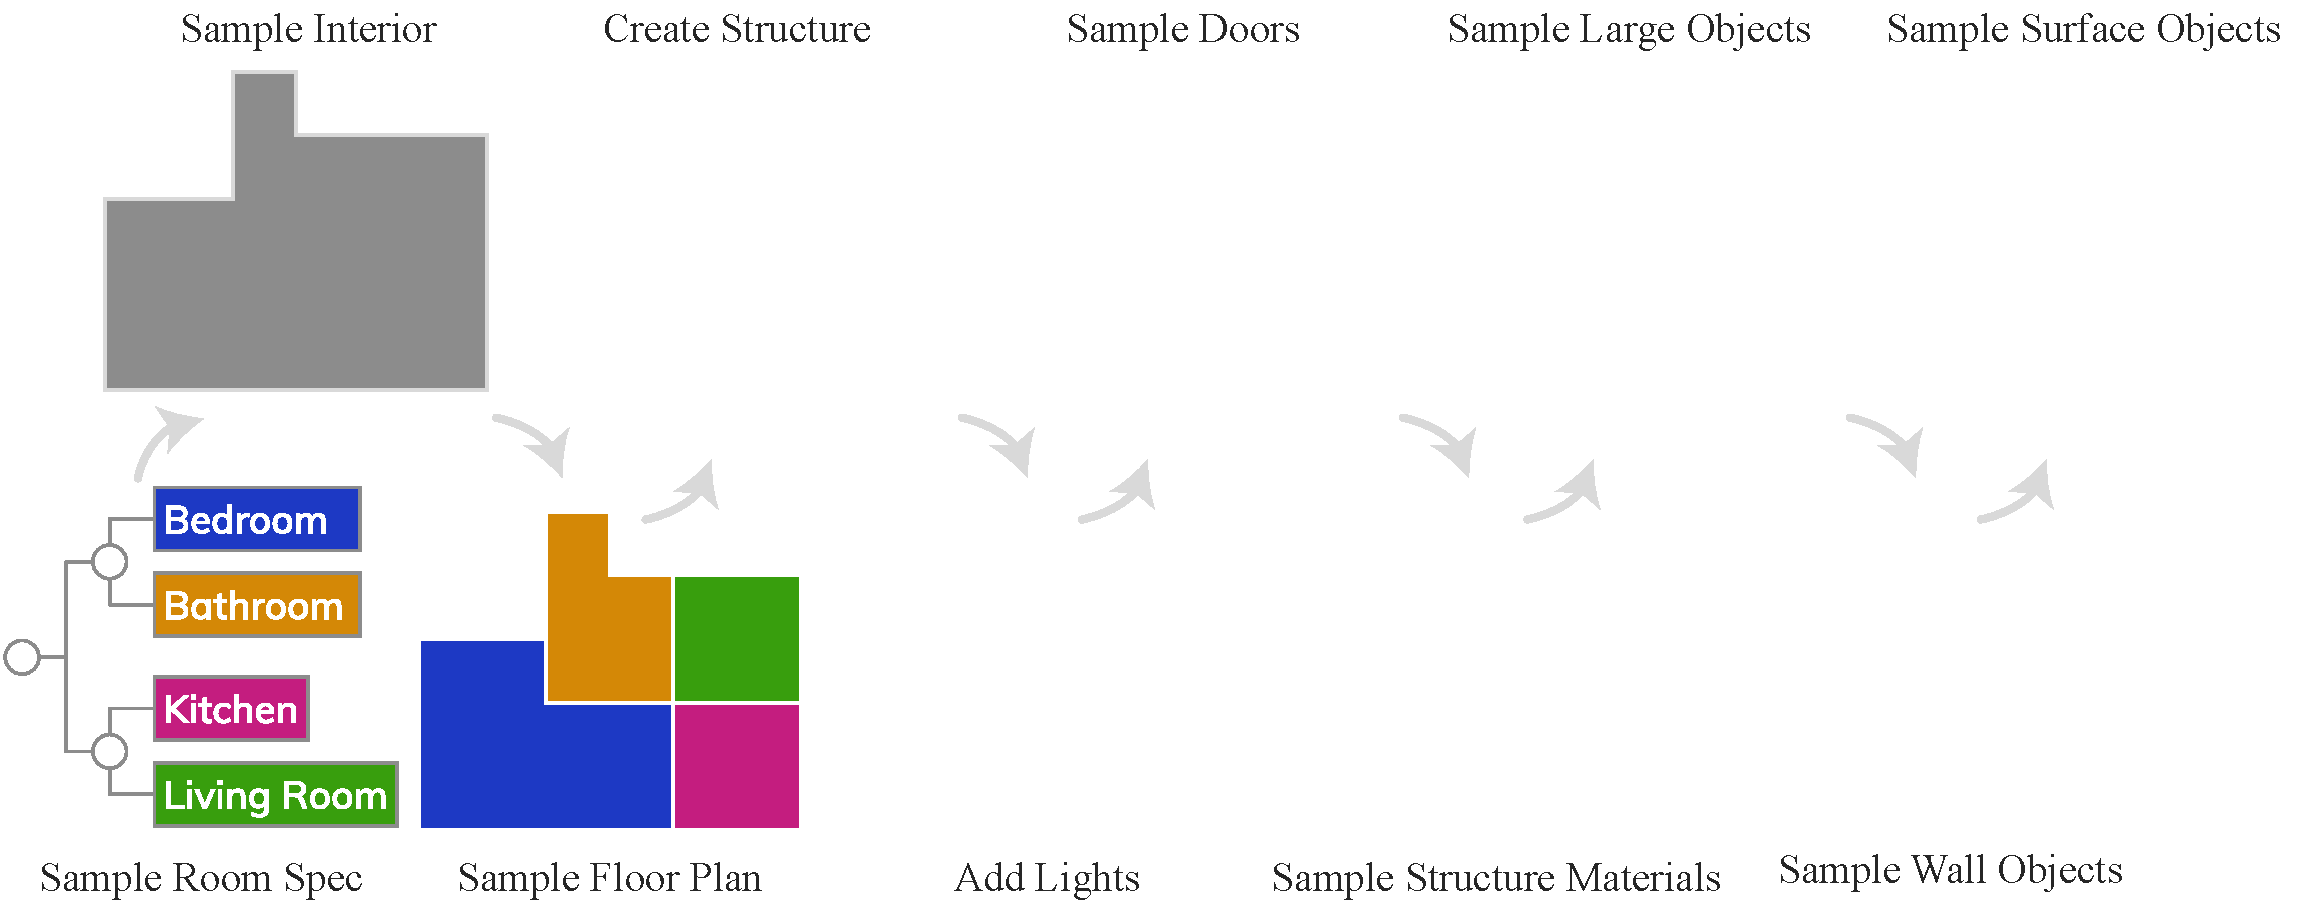
\includegraphics[width=1\textwidth]{figures/compressions/generation-3-vector.pdf}}
    \end{overpic}
    \captionof{figure}{Procedurally generating a house using \env.}
    \label{fig:genOverview}
\end{minipage}


Fig.~\ref{fig:genOverview} shows a high-level schematic of the procedure used by \env to generate a scene. Given a room specification (\eg house with 1 bedroom + 1 bathroom), \env uses multi-stage conditional sampling to, iteratively, generate a floor plan, create an external wall structure, sample lighting, and doors, then sample assets including large, small and wall objects, pick colors and textures, and determine appropriate placements for assets within the scene. We refer the reader to the appendix for details regarding our procedural generation and sampling mechanism, but highlight five key characteristics of \env: \textbf{Diversity}, \textbf{Interactivity}, \textbf{Customizability}, \textbf{Scale}, and \textbf{Efficiency}.

\noindent \textbf{Diversity.}
\env enables the creation of rich and diverse environments. Mirroring the success of pre-training models with diverse data in the vision and NLP domains, we demonstrate the utility of this diversity on several \eai tasks. Scenes in \env exhibit diversity across several facets:

\noindent \emph{Diversity of floor plans.} 
Given a room specification, we first employ iterative boundary cutting to obtain an external scene layout (that can range from a simple rectangle to a complex polygon). The recursive layout generation algorithm by Lopes \etal~\cite{lopes2010constrained} is then used to divide the scene into the desired rooms. Finally, we determine connectivity between rooms using a set of user-defined constraints. These procedures result in natural room layouts (e.g., bedrooms are often connected to adjoining bathrooms via a door, bathrooms more often have a single entrance, etc). As exemplified in Fig.~\ref{fig:floorplanExamples}, \env generates hugely diverse floor plans using this procedure.

\begin{minipage}{\linewidth}
    \centering
    \vspace{0.05in}
    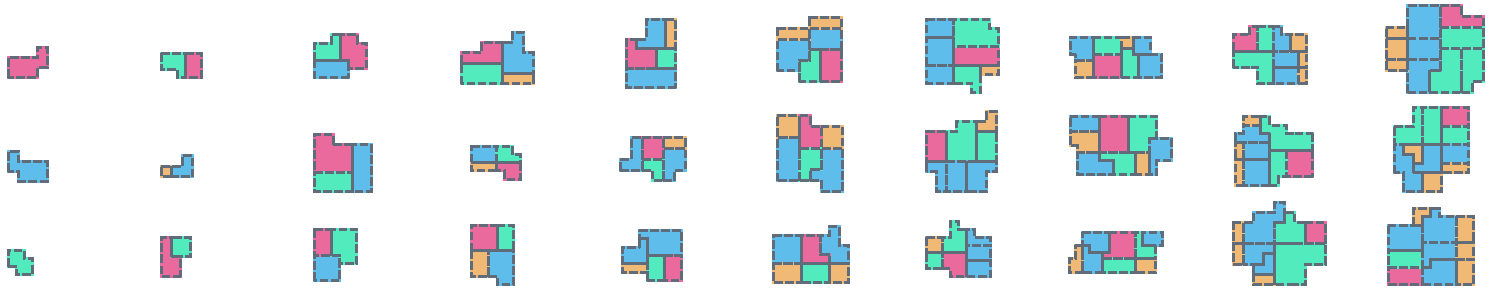
\includegraphics[width=0.9\textwidth]{figures/floorplans4_1.pdf}
    \captionof{figure}{\textbf{Floorplan diversity.} Examples showing the diversity of the generated floorplans. Rooms in the house are colored by \crule[bedroomColor]{2.5mm}{2.5mm} Bedroom, \crule[bathroomColor]{2.5mm}{2.5mm} Bathroom, \crule[kitchenColor]{2.5mm}{2.5mm} Kitchen, and \crule[livingRoomColor]{2.5mm}{2.5mm} Living Room.}
    \label{fig:floorplanExamples}
\end{minipage}

\noindent \emph{Diversity of assets.} 
\env populates scenes with small and large assets from its database of 1633 household assets across 108 categories (examples in Fig.~\ref{fig:assetsDiversity}). While many assets are inherited from \thor, we also introduce new assets such as windows, doors, and countertops, hand-designed by 3D graphic designers. Asset instances are split into train/val/test subsets and are interactable, i.e. objects can be picked and placed within the scenes, some objects have multiple states (\eg a light can be on or off) and several objects consists of parts with rigid body motions (\eg door on a microwave).

\begin{minipage}{\linewidth}
    \centering
    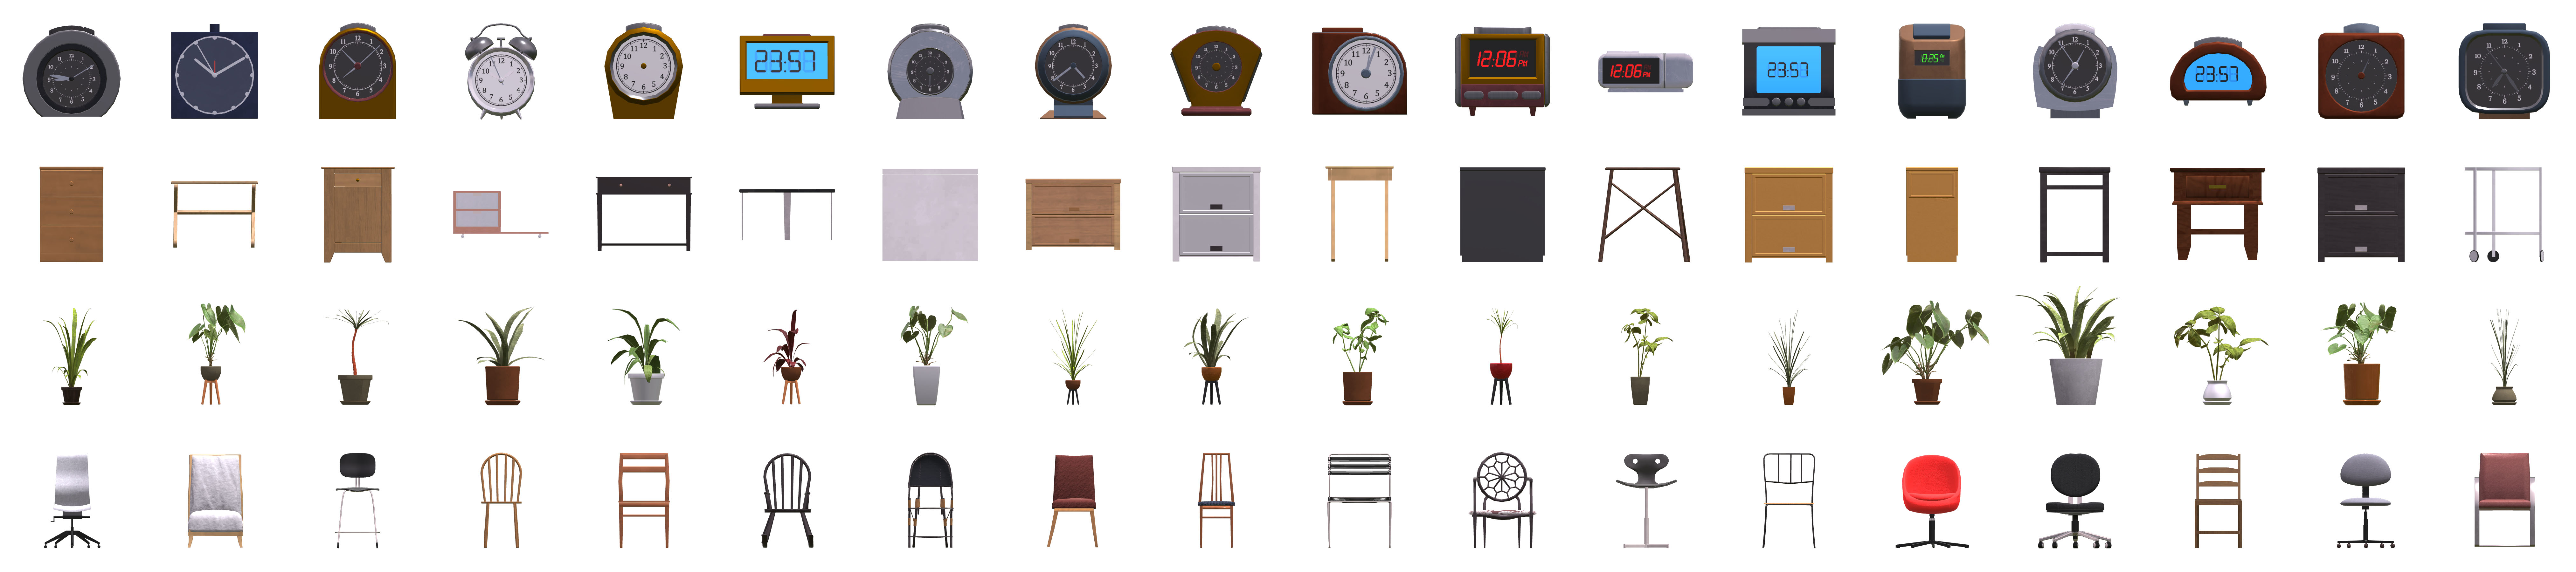
\includegraphics[width=1\textwidth]{figures/assets2.jpg}
    \begin{center}
        \vspace{-0.05in}
        {\large $\cdots$}
        \vspace{-0.05in}
    \end{center}
    
    \captionof{figure}{\textbf{Object diversity.} A subset of instances for four object categories.}
    \label{fig:assetsDiversity}
\end{minipage}

\noindent \emph{Diversity of materials.} 
Walls can have two kinds of materials -- one of 40 solid (and popular) colors or one of 122 wall textures such as brick and tile. 
% Rooms may have different wall colors/textures. 
We also provide 55 floor materials. The ceiling material for the entire house is sampled from the set of wall materials. \env also provides the ability to randomize materials of objects. Materials are only randomized within categories, which ensures objects still look and behave like the class they represent.

\begin{minipage}{\linewidth}
    \centering
    % \includegraphics[width=0.8\textwidth]{figures/textures-small2.jpg}
    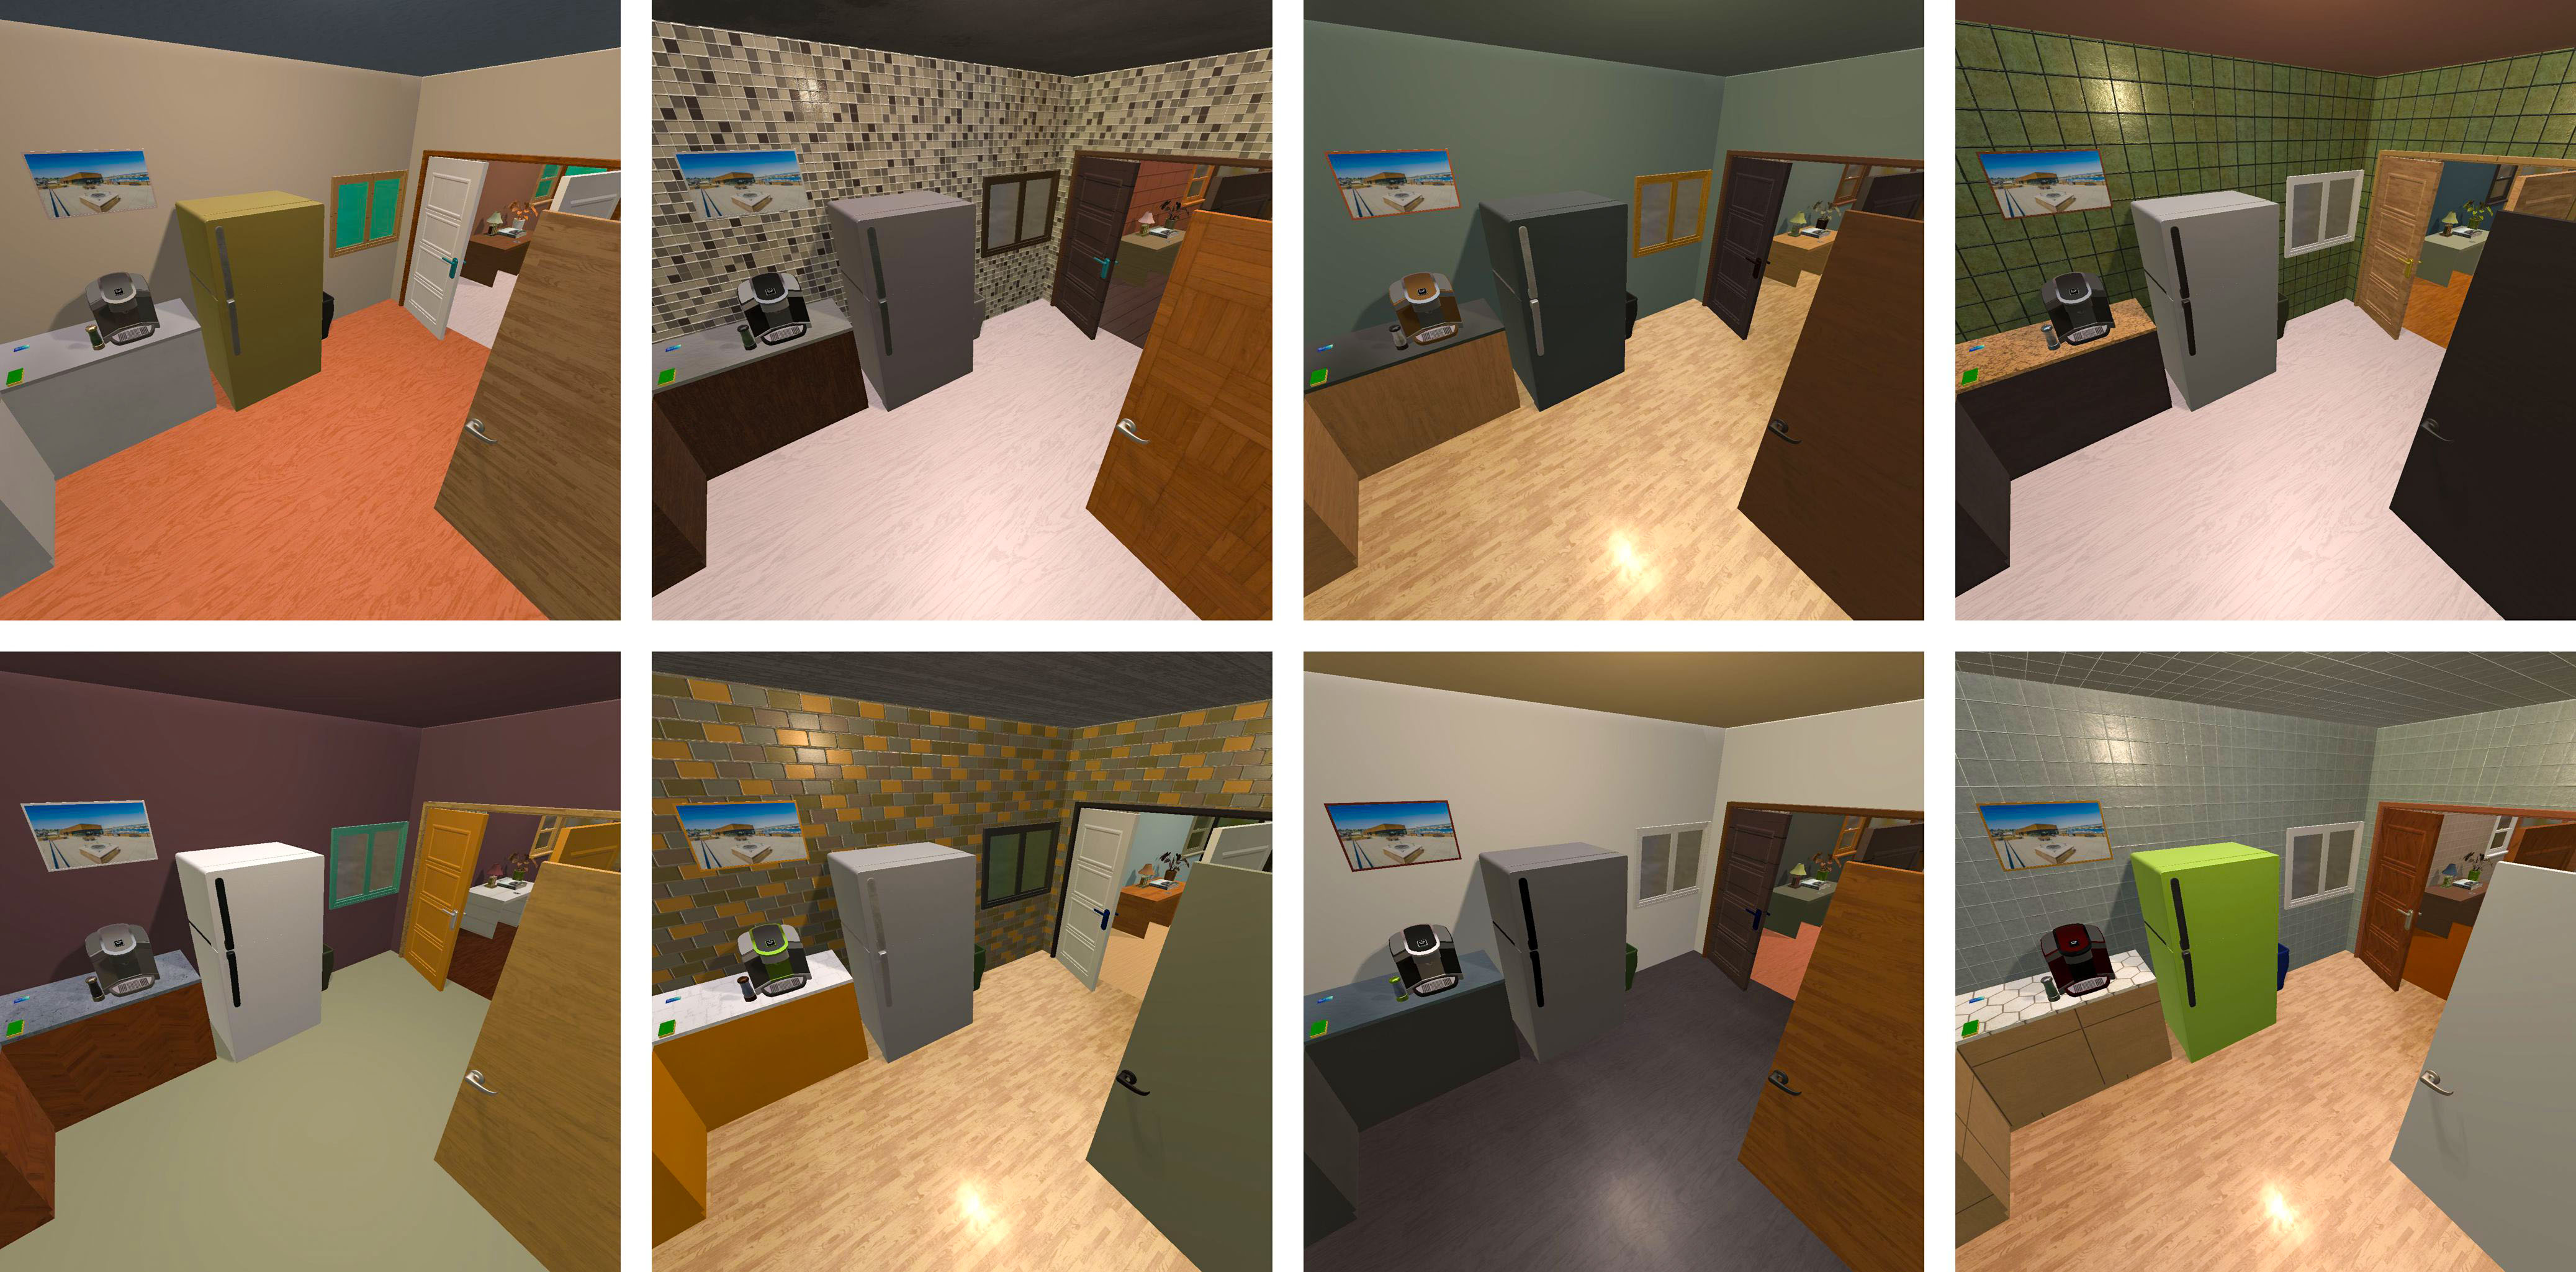
\includegraphics[width=1\textwidth]{figures/demo3.jpg}
    \captionof{figure}{\textbf{Material augmentation}. Different materials for objects and structural elements like walls and floors.}
    \label{fig:textureDiversity}
\end{minipage}



\noindent \emph{Diversity of object placements.} 
Asset categories have several soft annotations that help place them realistically within a house. These include room assignments (\eg couch in a living room but not a bathroom) and location assignments (\eg fridge along a wall, TV not on the floor). We also develop the notion of a Semantic Asset Group (SAG) -- groups of assets that typically co-occur (\eg dining table with four chairs) and thus must be sampled and placed using dependent sampling. Given a layout, individual assets and SAGs that lie on the floor are sampled and placed iteratively, ensuring that rooms continue to have adequate floor space for agents to navigate and manipulate objects. Then wall objects such as windows and paintings get placed, and finally, surface objects (ones found on top of other assets) are placed (\eg cups on the kitchen counter). This sampling allows for a large and diverse set of object choices and placements within any layout. Fig.~\ref{fig:placementDiversity} shows such variations.

\begin{minipage}{\linewidth}
    \centering
    \vspace{0.05in}
    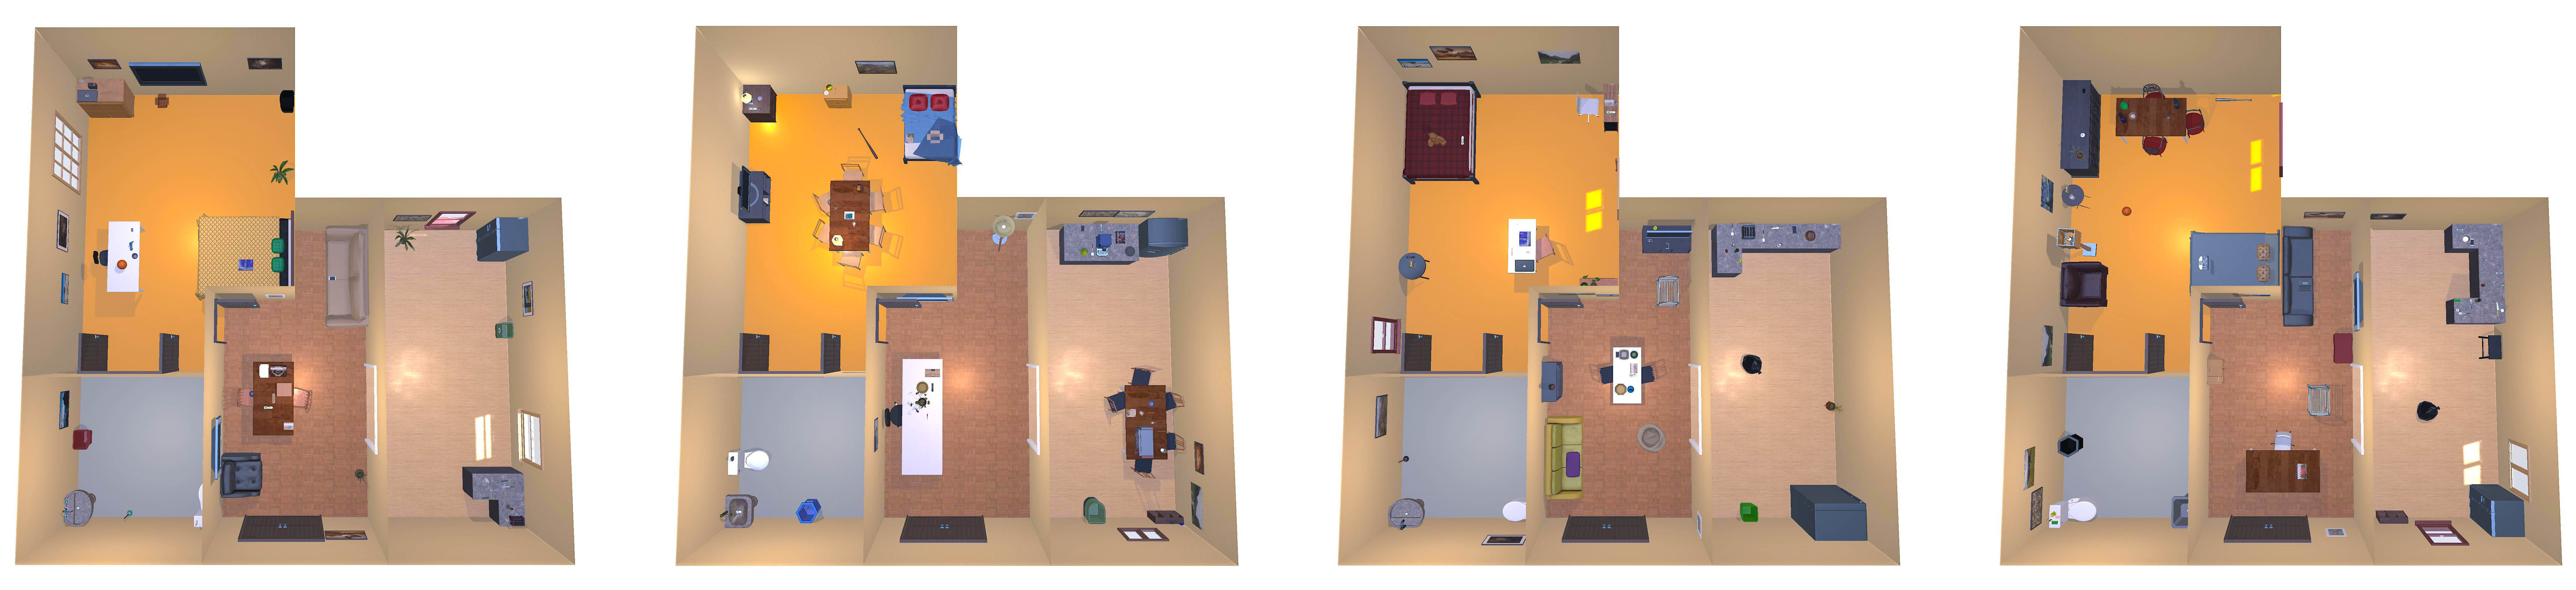
\includegraphics[width=1\textwidth]{figures/pos-placement-2.jpg}
    \captionof{figure}{\textbf{Object placement.} Four examples of object placement within the same room layout.}
    \label{fig:placementDiversity}
\end{minipage}

\noindent \emph{Diversity of lighting.}
\env supports a single directional light (analogous to the sun) and several point lights (analogous to lightbulbs). Varying the color, intensity, and placement of these sources allows us to simulate different artificial lighting, typically observed in houses, and also at different times of the day. Lighting has a significant effect on the rendered images as seen in Fig.~\ref{fig:lightingDiversity}.

\begin{minipage}{\linewidth}
    \centering
    \vspace{0.05in}
    
\includegraphics[width=1\textwidth]{figures/lighting-small2.jpg}
    \captionof{figure}{\textbf{Lighting variation}. Morning, dusk, and night lighting for an example scene.}
    \label{fig:lightingDiversity}
\end{minipage}

\noindent \textbf{Interactivity.} A key property of \env is the ability to interact with objects to change their location or state (Fig.~\ref{fig:interactivity}). This capability is fundamental to many Embodied AI tasks. Datasets like HM3D~\cite{Ramakrishnan2021HabitatMatterport3D} that are created from static 3D scans do not possess this capability. \env supports agents with arms capable of manipulating objects and interacting with each other.

\begin{minipage}{\linewidth}
    \centering
    \vspace{0.05in}
    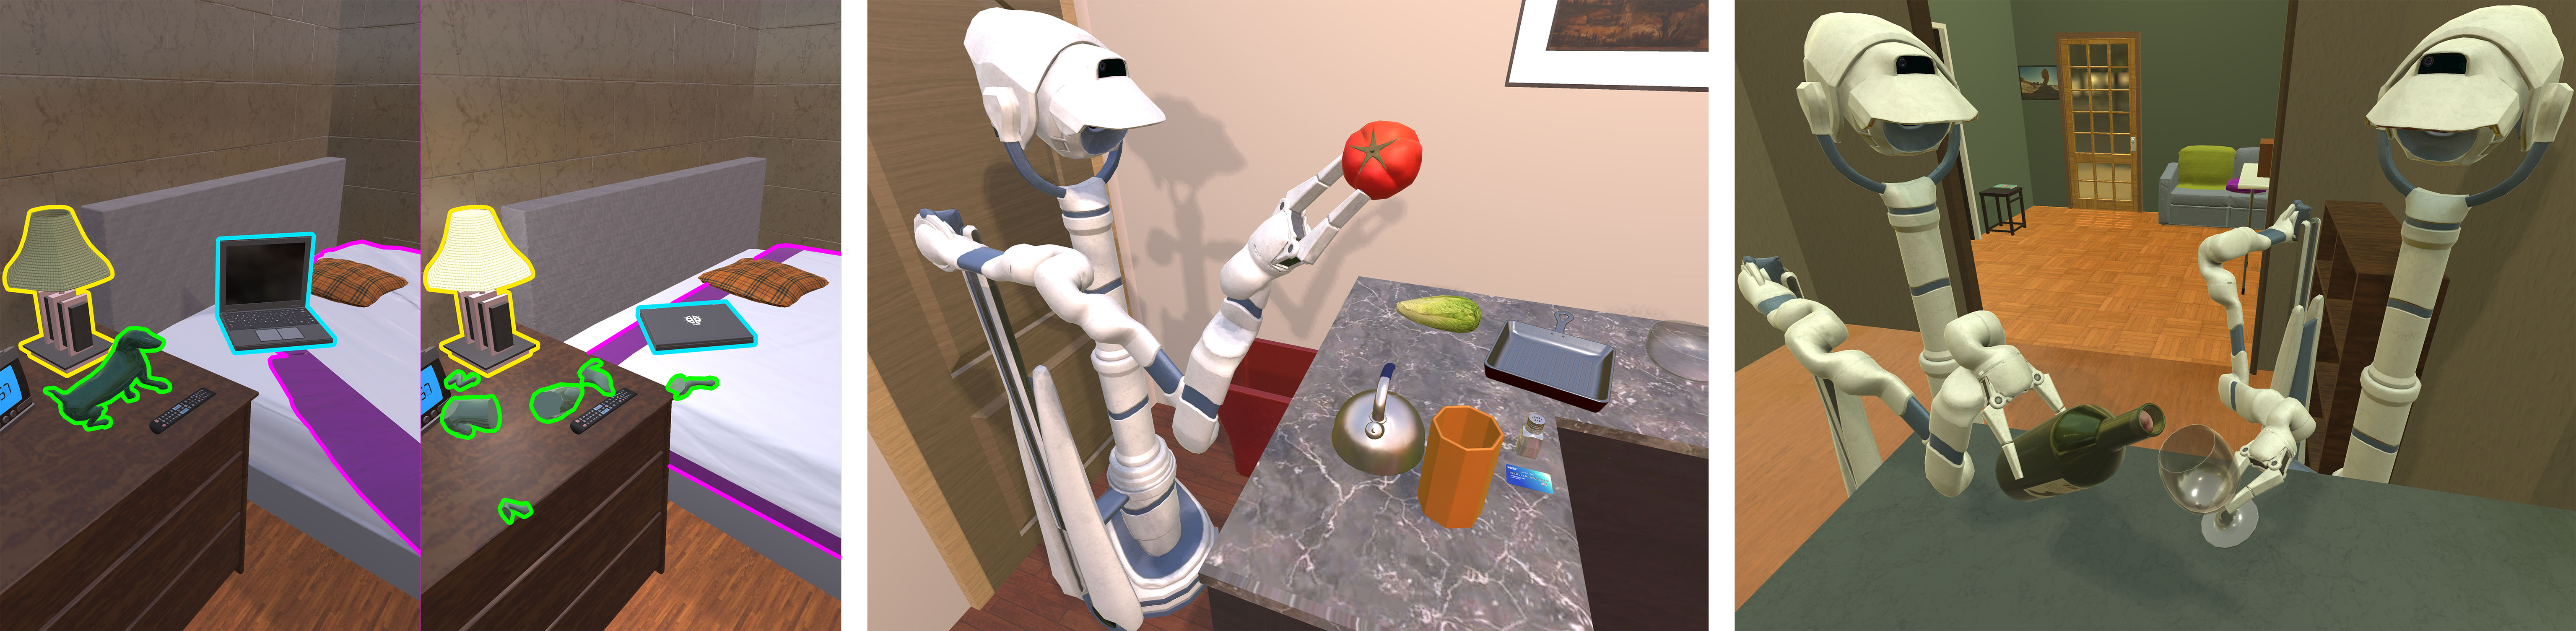
\includegraphics[width=1\textwidth]{figures/3PanelProcTHOR_03.jpg}
    \captionof{figure}{\textbf{Interactivity.} Object states can change (e.g., the laptop or the lamp in the left panel), and the agents can interact with objects and other agents (middle and right panels).}
    \label{fig:interactivity}
\end{minipage}

\noindent \textbf{Customizability.} \env supports many room, asset, material, and lighting specifications. With a few simple lines of specification, one can easily generate customized environments of interest. Fig.~\ref{fig:customize} shows examples of such varied scenes (classroom, library, and office).  

\begin{minipage}{\linewidth}
    \centering
    \vspace{0.05in}
    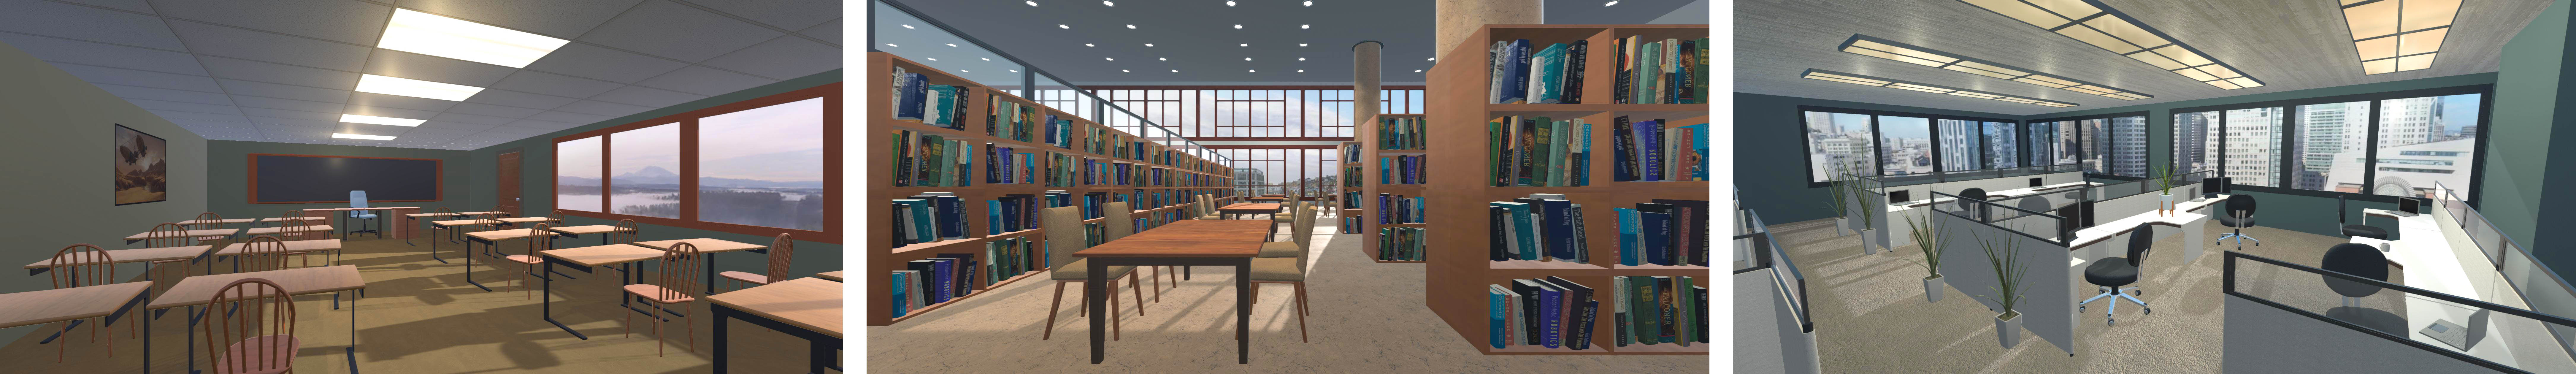
\includegraphics[width=1\textwidth]{figures/customizability.jpg}
    \captionof{figure}{\textbf{Customizability.} \env can be used to construct custom scene types such as classrooms, libraries, and offices.}
    \label{fig:customize}
\end{minipage}

\noindent \textbf{Scale and Efficiency.}
\env currently uses 16 different scene specifications to seed the scene generation process. These can result in over 100 billion layouts. \env uses 18 different Semantic Asset groups and 1633 assets. These can result in roughly 20 million unique asset groups. Each of these assets can be placed in numerous locations. In addition, each house gets scaled and uses a variety of lighting. This diversity of layouts, assets, materials, placements, and lighting enables the generation of \emph{arbitrarily large} sets of houses -- either statically generated and stored as a dataset or dynamically generated at each iteration of training. Scenes are efficiently represented in a JSON specification and are loaded into \thor at runtime, making the memory overhead of storing houses incredibly efficient. Moreover, the scene generation process is fully automatic and fast and \env provides high framerates for training \eai models (see Sec.~\ref{sec:analysis} for details).


% \todo{Reminder to mention there is zero annotation time for us compared to others.}